\chapter{Future work}

\section{Future instruments}

\subsection{\Ktwo}

\subsection{\TESS}

\subsection{\LSST}

The Large Synoptic Survey Satellite (LSST) is a 8.4 metre telescope with a 9.6
square degree field of view in Cerro Pach\'{o}n, Chile, currently under
construction.
It is designed to observe 18,000 square degrees in the southern sky (south of
+10 degrees, declination) in six Sloan Digital Sky Survey (\SDSS) filters:
ugrizy.
During its main mode of operation (90\% of the time), \LSST\ will perform two
fifteen second exposures per visit, with one thousand visits per night and
will have a faint limit of around 24.5 in r-band.
For the remaining 10\% of the time, \LSST\ will focus on a small number of
`deep drilling fields'.
These fields are yet to be determined but could be, for example, the Large and
Small Magellanic Clouds, the galactic plane, and so on.
These fields will receive targeted, repeat observations of, for instance 200
observations over a 40-hour period after which the faint limit could be
extended to around 28 apparent magnitudes (CITE THE WEBSITE?).
This faint limit will be extended for fields with co-added exposures.
First light is currently scheduled for 2021.
Data release one of eleven is expected to contain eighteen billion objects.

\LSST\ will provide rotation periods for a new stellar regime.
Because \kepler\ targeted Earth-like planet hosts, the majority of its
targets were G stars, with fewer K and M dwarfs.
Since the collecting area of \LSST\ is so large it will be sensitive to a
large number of faint stars, including many K and M dwarfs.
Since it is not a space mission and its lifetime does not depend on the
reliability of moving parts or fuel, \LSST\ will run for 10 years---more than
double the length of the \kepler prime mission.
This will open up an opportunity to detect rotation signatures in faint,
slowly rotating stars, allowing us to populate both the low-mass and old parts
of the age-rotation parameter space.
In many ways \LSST\ is \kepler's antithesis: \kepler data is dense and evenly
spaced, whereas \LSST\ light curves will have sparse, irregular cadence.
Depending on its location on the sky, a given target will have between ... and
... data points spread over 10 years, spaced from 3 days to 30 days apart.
The disadvantage of this is that there will be a rotation period lower limit.
The advantage of using sparse data however, is that CPU time is vastly
reduced!

We simulated \LSST cadence by requiring that an object/field only be observed
during the night and whilst the field is visible, so for half of the year.
Each object is visited every three days, on average during the observable
season and visits are clustered around a season with a Gaussian shape.
A histogram of the number of visits per week as a function of time for a given
object or field is shown in figure \ref{fig:cadence_hist}.

\begin{figure}
\begin{center}
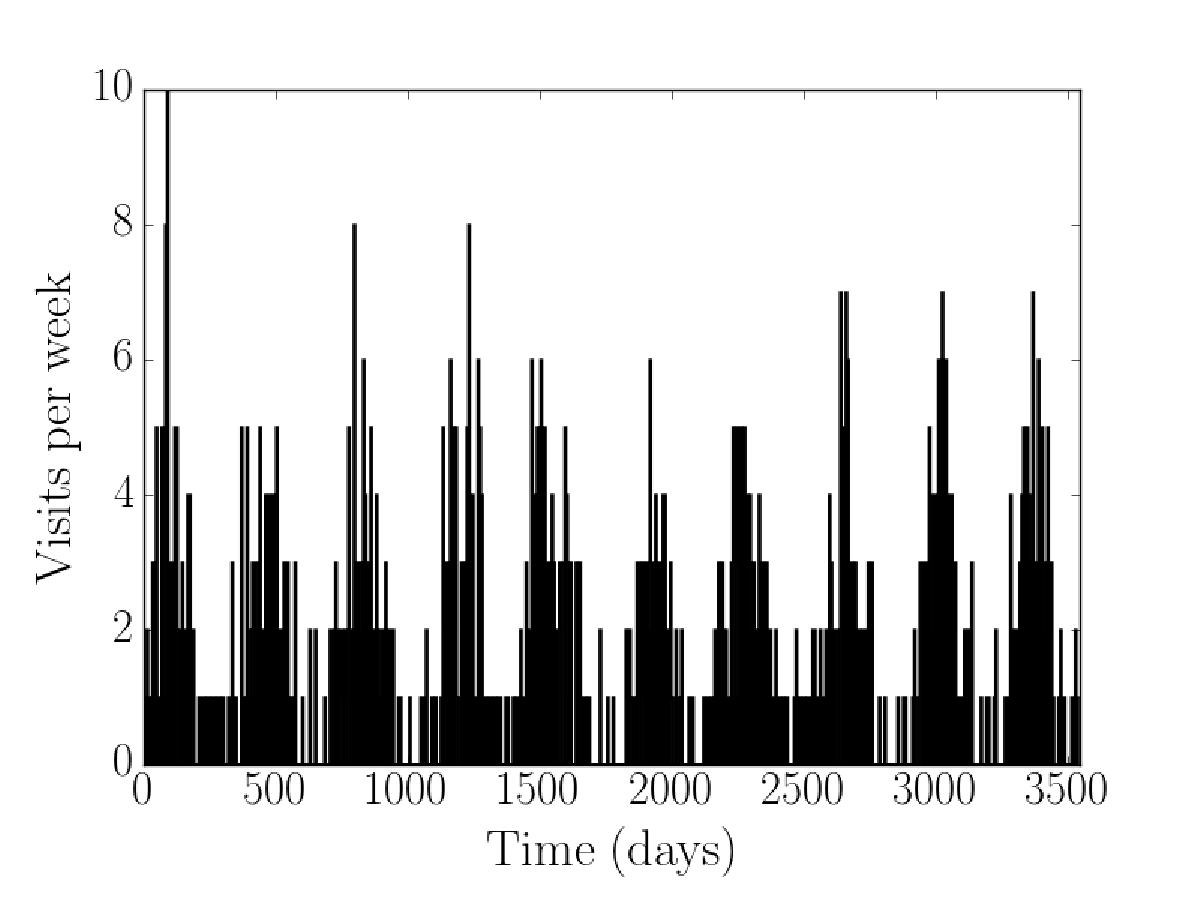
\includegraphics[width=6in, clip=true]{figures/cadence_hist}
\caption[An LSST cadence histogram.]
{A histogram of the number of visits per week as a function of time
for a given object or field observed by \LSST as used in our simulations.}
\label{fig:cadence_hist}
\end{center}
\end{figure}

Since \LSST observations are not evenly spaced, it is not trivial to compute
an autocorrelation function.
(LOOK UP COLLIER-CAMERON AND MAZEH)
One could interpolate the light curve onto an evenly spaced grid and then
compute the ACF, but this would introduce a large amount of uncertainty.
Instead of using an ACF to initialise our MCMC we therefore use the
Lomb-Scargle periodogram.

\subsection{\PLATO}

\section{Future projects}

information, so these will be used too) and will be tested on binary stars.
In addition to the basic input catalogues available for the transit survey
stars, I will gather information from every other available source.
Light curves themselves are rich in age information, for example, even where
a rotation period cannot be measured, the {\it absence} of discernable
variability is indicative of old-age.
I will use the method of \citet{bastien} to measure short-timescale brightness
fluctuations (known as flicker) which are correlated with surface gravity.
I will also use new distance and proper motion information from GAIA as soon as
the data become available (expected in early 2017).
To obtain accurate gyrochronological ages, reliable rotation periods must be
inferred---this is another challenge which has prohibited the exploration of
time-dependent exoplanet populations thus far.
Standard methods for rotation period inference such as autocorrelation
functions (ACFs) and sine-fitting periodograms are not optimal for noisy light
curves with low-amplitude signals, are not probabilistic, do not provide
realistic uncertainties and are performed on `detrended' \Kepler\ light curves
with significantly reduced power at periods of 30 days and above.
My new technique for measuring probabilistic rotation periods using Gaussian
processes (GPs) can extract rotation periods from low-amplitude signals that
are buried in noisy data, can be applied directly to unprocessed light curves
and measures more precise and accuration rotation periods than ACF and
periodogram methods \citep{AngusIAU}, see figure \ref{fig:rotation}.
I will use this method to compute a probabilistic constraint on the rotation
periods of {\it all} transit survey stars.

This new dating method will be probabilistic---hierarchical Bayesian inference
will be performed in order to `learn' an informative age prior from the data
themselves; a prior that will reflect the most probable age of a star, given
the age distribution of other stars observed.

There are several advantages to this dating model.
Firstly, combining all the information will provide more precise and accurate
ages than any one method used on its own, and, by definition, these ages will
be less dependent upon one single model.
Secondly, it will provide an age constraint for every star observed by
a photometric survey since {\it some} age information is always available.
Thirdly, it will be directly compatible with my probabilistic, GP rotation
period measurement method and finally, it will be easily updated as new data
become available.
By modelling stellar ages using all available information and combining
multiple dating techniques, my hierarchical, Bayesian dating method with
informative priors {\bf will provide the most precise and accurate ages ever
inferred for every star observed by \Kepler, \Ktwo\ and \TESS}.

This project is highly ambitious and will have enormous impact if successful,
however even if there is no detectable age-trend in the \Kepler\ data it will
lead to other discoveries and useful products for the astronomical
community.
Firstly, a rotation period and age for every \Kepler, \Ktwo\ and \TESS\ star
will be beneficial to both exoplaneteers and galactic archaeologists alike,
\citep[e.g.][]{bovy}.
Secondly, stellar rotation periods can reveal potential star-planet
interactions in which a planet transfers angular momentum to its host---I
intend to unambiguously confirm this phenomenon.
Finally, this work will pave the way for exoplanet-age studies with PLATO.
Launching in 2025, this space telescope will provide highly precise
asteroseismic ages for thousands of stars, revolutionising the field of
stellar ages.

